\def\col{blue}
\documentclass[14pt, \col, hyperref={pdfpagelabels=false}]{beamer}
\usepackage[frenchb]{babel} % langue francaise
\usepackage[utf8]{inputenc} % encodage UTF-8
\usepackage[T1]{fontenc} % encodage de la police de caracteres
\usepackage{lmodern}
\usepackage{listings}
\usepackage{multicol}
\usepackage{pifont} %\ding{number}, 
\usepackage{subfigure}
\usepackage{graphicx}
\usepackage{listings}

\usetheme{Warsaw}
\usepackage[\col]{optional} %red blue green
%% THÈMES couleur
%% \usecolortheme{dolphin}
%% \usecolortheme{seahorse}
%% * thèmes globaux : beetle, crane, fly, seagull.
%% * thèmes internes : lily (enlève surtout des couleurs), orchid, rose.
%% * thèmes externes : whale, seahorse, dolphin

% rubber: rules ./rules.ini

 
\mode<presentation>
{
  %%%% Couleurs
  \definecolor{red2}{rgb}{0.8,0.15,0.15}
  \definecolor{bx}{rgb}{0.45,0.05,0.05}  
  \definecolor{ivoire}{rgb}{1, 0.97, 0.9}
 
  \definecolor{bleu2}{rgb}{0.9, 0.90, 1}
  \definecolor{bleu3}{rgb}{0.15,0.15,0.7}
  \definecolor{myblue}{rgb}{0.50,0.55, 0.8}  
  \definecolor{myblue2}{rgb}{0.25,0.3, 0.65}  
  
 \definecolor{mygreen2}{rgb}{0.15,0.60,0.15}
 \definecolor{green2}{rgb}{0.15,0.40,0.15}
  \definecolor{mygreen}{rgb}{0.40,0.7, 0.4}  
%  \definecolor{lightgreen}{rgb}{0.5,0.8, 0.5}  
  \definecolor{lightgreen}{rgb}{0.95, 1, 98}
  
  \definecolor{medium-grey}{gray}{0.45}
  \definecolor{light-grey}{gray}{0.85}
  
  % Couleur des structures et fond dégradé
  % defaut: green
  \setbeamercolor{normal text}{fg=black,bg=lightgreen}
  \setbeamercolor{structure}{fg=green2, bg=light-grey} 
  \setbeamercolor{alerted text}{fg=green2}
  \setbeamertemplate{background canvas}[vertical
    shading][top=lightgreen!100,bottom=lightgreen!30]
  
  \opt{blue}{
    \setbeamercolor{normal text}{fg=black,bg=bleu2}
    \setbeamercolor{structure}{fg=myblue, bg=light-grey} 
    \setbeamercolor{alerted text}{fg=myblue2}
    \setbeamertemplate{background canvas}[vertical
      shading][top=bleu2!100,bottom=bleu2!30]
  }
  \opt{red}{
    \setbeamercolor{normal text}{fg=black,bg=ivoire}
    \setbeamercolor{structure}{fg=bx, bg=light-grey} 
    \setbeamercolor{alerted text}{fg=red2}
    \setbeamertemplate{background canvas}[vertical
      shading][top=ivoire!40,bottom=ivoire!100]
  }
  \opt{green}{
    \definecolor{green2}{rgb}{0.1,0.60,0.1}
    \usecolortheme{dolphin}
  }   
  
  
  \setbeamertemplate{navigation symbols}{}
  \setbeamerfont{title in head/foot}{size=\scriptsize}
  \setbeamerfont{date in head/foot}{size=\scriptsize} 
  
  % Pied de page
  \setbeamertemplate{footline}{
    \hbox{%
      \begin{beamercolorbox}[wd=.4\paperwidth,ht=3ex,dp=1ex,center]{title in head/foot}
        \usebeamerfont{title in head/foot}\enseignement\hspace{1cm} %\shorttitle
      \end{beamercolorbox}%
      \begin{beamercolorbox}[wd=.5\paperwidth,ht=3ex,dp=1ex,left]{date in head/foot}%
        \usebeamerfont{title in head/foot} 
        \hspace*{1ex} 
        \insertshorttitle
      \end{beamercolorbox}% 
      \begin{beamercolorbox}[wd=.1\paperwidth,ht=3ex,dp=1ex,left]{date in head/foot}%
        \usebeamerfont{date in head/foot} 
        \insertframenumber{} / \inserttotalframenumber%\hspace*{2ex} 
    \end{beamercolorbox}}%
    \vskip0pt%
  }

    % Haut de page
  \setbeamertemplate{headline}{%
    \leavevmode
    \begin{beamercolorbox}[wd=.5\paperwidth,ht=3ex,dp=1.125ex,leftskip=.3cm
        plus1fill,rightskip=.3cm]{section in head/foot}%
      \scriptsize{\insertsection}
    \end{beamercolorbox}%
    \begin{beamercolorbox}[wd=.5\paperwidth,ht=3ex,dp=1.125ex,leftskip=.3cm,rightskip=.3cm
        plus1fil]{subsection in head/foot}%
      \scriptsize{\insertsubsection}
    \end{beamercolorbox}%
  }
  \addtobeamertemplate{headline}{}{%
    \vskip-0.1pt
    \pgfuseshading{beamer@topshade}
    \vskip-2pt}
   %% \let\Tiny=\tiny
  %% \let\TINY=\tiny
}

%% Annonce de plan a chaque transition.
%% \AtBeginSection[]{
%%   \begin{frame}<beamer>
%%     \frametitle{Plan}
%%     \tableofcontents[currentsection,currentsubsection]
%%   \end{frame}
%% }



\newcommand{\bashlisting}[0]{\scriptsize\lstset{language=bash,numbers=left,numberstyle=\tiny,
    xrightmargin=1mm, xleftmargin=1mm, keywordstyle=\color{green2}, %
    keywordstyle[1]=\color{blue}, %
    keywordstyle[2]=\color{yellow}, %
    keywordstyle[3]=\color{red2}}}

\newcommand{\filelisting}[0]{\small\lstset{language=,numbers=left,numberstyle=\tiny,
    xrightmargin=4mm, xleftmargin=6mm, frame=single}}

\definecolor{orange}{rgb}{0.9,0.6,0.4}

\newcommand{\clisting}[0]{\scriptsize
  \lstset{language=c, 
    inputencoding=utf8,
    %identifierstyle=\color{blue},%
    keywordstyle=\color{green2}, %
    keywordstyle[1]=\color{blue}, %
    keywordstyle[2]=\color{yellow}, %
    keywordstyle[3]=\color{red2}, %
    stringstyle=\color{orange}, %
    commentstyle=\color{red2}, %
    numbers=left,
    numberstyle=\tiny,
    xleftmargin=1mm,
    breaklines=true,
}}



\newcommand{\cmd}[1]{\texttt{\footnotesize\textcolor{medium-grey}{#1}}}

\newcommand{\cmdlist}[1]{
  \begin{semiverbatim}\begin{minipage}{\linewidth}  
      \footnotesize\textcolor{medium-grey}{#1}\end{minipage}
\end{semiverbatim}}


\newcommand{\coeur}{c\oe ur\xspace}
\newcommand{\oeuvre}{\oe uvre\xspace}
\newcommand{\coeurs}{c\oe urs\xspace}
\newcommand{\mc}{multic\oe ur\xspace}
\newcommand{\mcs}{multic\oe urs\xspace}

\usepackage{multicol}

%%%%%%%%%%%%%
\def\enseignement{ASR2 Système}
\title[]{\enseignement\\
  Stockage des fichiers}
\author{Stéphanie Moreaud}
\institute{Département d'informatique\\
  IUT Bordeaux 1}
\date{}
   
%%%%%%%%%%%% 
   
\newcommand{\TITRE}[1]{
  \begin{frame} \begin{center}\huge{#1}\end{center}
\end{frame}
}
\newcommand{\FIGURE}[2]{
  \begin{frame} \frametitle{\insertsubsection} 
    \begin{figure} \includegraphics[width=0.8\linewidth]{fichiers-images/#1} 
    \end{figure} 
    \begin{center}\large{#2}\end{center}
\end{frame} }

%%%%%%%%%%%%%%%%%%%%%%%%%%%%%%%%%%%%%
\begin{document}
\begin{frame}
  \titlepage
\end{frame}

\begin{frame}<beamer>
  \frametitle{Plan} \begin{columns}[t] \begin{column}{5cm} \tableofcontents[sections={1-5},currentsection,
  hideothersubsections] \end{column} \begin{column}{5cm} \tableofcontents[sections={6-10},currentsection,hideothersubsections] \end{column} \end{columns}
\end{frame}
%Annonce de plan a chaque transition.
\AtBeginSection[]{
  \begin{frame}<beamer> 
    \frametitle{Plan}
    \begin{columns}[t] 
      \small
      \begin{column}{6cm} 
        \tableofcontents[sections={1-4}, currentsection, hideothersubsections] 
      \end{column} 
      \begin{column}{5cm} 
        \tableofcontents[sections={5-10},currentsection,hideothersubsections] 
  \end{column} 
  \end{columns} 
    \normalsize
  \end{frame}
    }

\begin{frame}
\frametitle{Bibliographie}
\bibliographystyle{fr-plain}
\small
\nocite{*}    
\bibliography{bib} 
\vspace{0.5cm}    
D'après les transparents de Michel Billaud.
\end{frame}
%%%%%%%%%%%%%%%%%%%%%%%%%
%%%%%% Let's go!  %%%%%%
%%%%%%%%%%%%%%%%%%%%%%%%%

\section{Rappel}
\subsection{Système d'exploitation}
\begin{frame}
\frametitle{Qu'est ce qu'un système d'exploitation~?}
Un \alert{Système d'Exploitation} (\emph{Operating System}) est une
\alert{couche d'abstraction} (ensemble de programmes) construite au dessus du matériel pour
\begin{itemize}
\item masquer la complexité du matériel
\item arbitrer l'accès aux ressources
\begin{itemize}
\item \normalsize{processeurs, mémoire, périphériques, ...}
\end{itemize}
\end{itemize}
\end{frame}

\subsection{Ordonnancement de processus}
\begin{frame}
\frametitle{Utilisation du processeur}
Dans un système des \alert{processus} (instance de programmes en cours d'exécution) 
sont exécutés par le(s) processeur(s). \\
\vspace{0.5cm}
Arbitrage de l'occupation CPU par l'\alert{ordonnanceur}. 
\vspace{0.5cm}

Évolution des systèmes
\begin{itemize}
\item monotâche
\item monotâche avec traitement par lot
\item multiprogrammation, temps partagé
\item multitâche
\end{itemize}
\end{frame}


\begin{frame}
\frametitle{Utilisation du processeur} 
Ordonnancement \ding{212} choix du processus à exécuter.\\
\vspace{0.5cm}
Plusieurs stratégies d'ordonnancement possibles selon les systèmes
\begin{itemize}
\item FIFO, PCTE, priorité, ...
\end{itemize}
\vspace{0.5cm}

Systèmes multitâches
\begin{itemize}
\item systèmes coopératifs (sans réquisition)
  \begin{itemize}
  \item profite des ``temps morts'' 
  \end{itemize}
\item systèmes avec préemption
  \begin{itemize}
  \item notion d'interruption, quantum. 
  \end{itemize}
\end{itemize}
\end{frame}

\subsection{Gestion de la mémoire}
\begin{frame}
  \frametitle{Gestion de la mémoire}
  Plusieurs programmes chargés en mémoire
  \vspace{0.5cm}
  \begin{itemize}
  \item code indépendant de sa position en mémoire
    \normalsize{
      \begin{itemize}
      \item notion d'adresse logique
      \item convertie par le système en adresse physique
      \end{itemize}}
  \vspace{0.5cm}
  \item gestion de l'espace mémoire
    \normalsize{
      \begin{itemize}
      \item allocation/restitution 
      \item protection
      \end{itemize}}
  \end{itemize}
\end{frame}

\begin{frame}
  \frametitle{\insertsubsection}
  \alert{Allocation contiguë}
  \begin{itemize}
  \item problème de fragmentation 
  \item diverses stratégies~: Fisrt-fit, Best-fit, etc.
  \item compactage (solution curative)
  \end{itemize}
  \alert{Segmentation} 
  \begin{itemize}
  \item division de l’espace mémoire en segments logiques
  \item partage de segments (code, bibliothèque), économie mémoire, etc.
  \item adresse logique comprend un numéro de segment, utilisation d'une table des segments
  \end{itemize}
\end{frame}

\begin{frame}
\frametitle{\insertsubsection}
\alert{Pagination}
  \begin{itemize}
  \item espace découpé en pages de mêmes tailles
  \item chargées en mémoire dans des cadres de pages, pas forcément consécutifs
  \item conversion adresse logique/physique grâce à la table des pages
  \item stratégies de remplacement des pages 
  \end{itemize}
\alert{Swapping (va-et-vient)}
  \begin{itemize}
  \item mémoire rarement suffisante pour maintenir tous les processus 
  \item échanges entre le disque et la mémoire
  \end{itemize}
\end{frame}


\begin{frame}
  \frametitle{\insertsubsection}
  Utilisation combinée de la segmentation, pagination et du swapping.
  \begin{itemize}
  \item[\ding{212}] mémoire virtuelle paginée 
  \item circuit matériel spécialisé, MMU (\emph{Memory Managment Unit})
  \item processus partiellement chargés en mémoire
  \item rapatriement des pages au besoin (défaut de pages) 
  \end{itemize}
\end{frame}



\section{Introduction}
\begin{frame}
\frametitle{\insertsection}
Le système d'exploitation doit masquer les particularités 
des disques et autres périphériques d'entrée/sorties. \\
\vspace{0.5cm}
Comment prend t-il en charge les accès disques?
\vspace{0.5cm}
\begin{itemize}
\item Données organisées sous la forme de \alert{fichiers}.
\item Comment fonctionne un disque? \\
  Quelles spécificités faut-il prendre en compte?\\
  Comment assembler des disques pour améliorer capacité et fiabilité?
\item Système de gestion des fichiers.
\end{itemize}
\end{frame}



%%%%%%%%%%%%%%%%%%%%%%%%%%%%%%%%%%%%%%%%%%%%%%%%%%%%%%%%%%%%%%%%%%%%%%%%%%%%%%%%%%%%%%%%%
\section{Fichiers}
\begin{frame}
  \frametitle{Qu'est-ce qu'un fichier~?}
  Un \alert{fichier} est un \alert{lot d'informations} portant un nom et conservé dans
  une mémoire. \\
  \begin{itemize}
  \item une suite de bits codant de l'information
    \texttt{\center{01101001 01001010 0100100 10010010 0001010 11010101
        10101011 01101001 ...}}
  \end{itemize}
\end{frame}

\begin{frame}
  \frametitle{Qu'est-ce qu'un fichier~?}
  Les fichiers sont la plupart du temps \structure{conservés sur} des mémoires de
  masse tels que les \structure{disques durs}.\\
  \vspace{0.5cm}
  Les fichiers sont classés dans des \structure{répertoires}
  \begin{itemize}
  \item chaque répertoire peut contenir d'autres répertoires
  \end{itemize}
  \ding{212} \structure{organisation arborescente} appelée \alert{système de fichiers}.
\end{frame}

\begin{frame}
\frametitle{Système de fichiers}
\vspace{-0.2cm}
\begin{figure}
  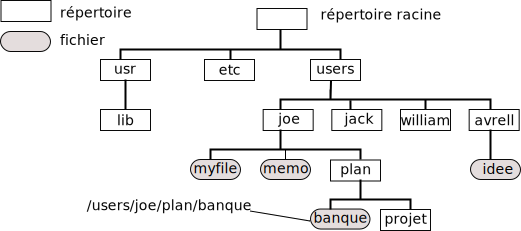
\includegraphics[width=\linewidth]{fig3/file_sys}
\end{figure}
\end{frame}


%% \begin{frame}
%% \frametitle{Contenu du cours}
%% \begin{itemize}
%% \item Comment marche un disque
%% \item La gestion d'un disque par le système
%% \item les systèmes RAID
%% \item l'organisation des fichiers sur disque
%% \item les arborescences
%% \end{itemize}
%% \end{frame}

%%%%%%%%%%%%%%%%%%%%%%%%%%%%%%%%%%%%%%%%%%%%%%%%%%%%%%%%%%%%%%%%%%
\section{Disques}

\subsection{Qu'est ce qu'un disque?}

\begin{frame}
\frametitle{\insertsubsection}
\vspace{-0.1cm}
\begin{figure}
  \includegraphics[width=0.8\linewidth]{fig3/magnetic-drum.jpeg}
 \end{figure}
\vspace{-0.1cm}
 Ancêtre~: le tambour magnétique
\end{frame}

\begin{frame}
\frametitle{\insertsubsection}
\begin{multicols}{2}
\begin{minipage}[t]{1\linewidth}
\begin{figure}
  \vspace{-1cm}
  \includegraphics[width=1.1\linewidth]{fig3/5MB-Hard-Disk-in-1956.png}
\end{figure}
\end{minipage}
\vspace{2cm}
\center Moins récent (1956),\\
capacité 5Mo. 
\end{multicols}
\end{frame}

\begin{frame}
  \frametitle{\insertsubsection}
  \begin{multicols}{2}
    \begin{minipage}[t]{1.4\linewidth}
    \vspace{-1cm}
      \begin{figure}
        \includegraphics[width=1\linewidth]{fig3/DiamondMax-80GB-Internal-Hard-disk.png}
      \end{figure}
    \end{minipage}
    \hspace{2cm}
    \begin{minipage}[t]{\linewidth}
      \vspace{2cm}
    \center ~~~~~~~~~~~~~Disque récent,\\ 
     ~~~~~~~~~~~~~capacité 80Go. 
    \end{minipage}
  \end{multicols}
\end{frame}

\subsection{Disque, tête}
\begin{frame}
  \frametitle{\insertsubsection}
  \begin{figure}
    \includegraphics[width=0.8\linewidth]{fig3/tete-lecture.png}
    \center{Disque, tête de lecture, bras}
  \end{figure}
\end{frame}
  

\begin{frame}
  \frametitle{\insertsubsection}
  Données stockées sous forme de bits sur une fine couche magnétique
  \begin{itemize}
  \item quelques microns d'épaisseur
  \end{itemize}
  
  \vspace{0.5cm}
  Lecture et l'écriture faite par une tête de lecture 
  \begin{itemize}
  \item électro-aimant
  \item se baisse/soulève pour lire/écrire l'information
  \end{itemize}
\end{frame}


\begin{frame}
  \frametitle{\insertsubsection}
  La position d'une tête définit une \alert{piste}
  \begin{figure}
    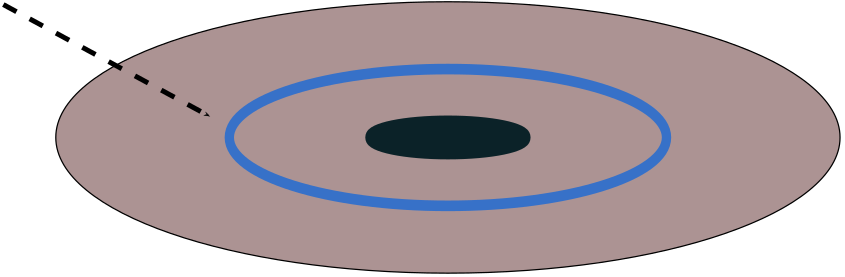
\includegraphics[width=0.8\linewidth]{fig3/piste}
    \center{Une piste}
  \end{figure}
\end{frame}

\begin{frame}
  \frametitle{\insertsubsection}
  Les pistes sont découpées en \alert{secteurs}
  \begin{figure}
    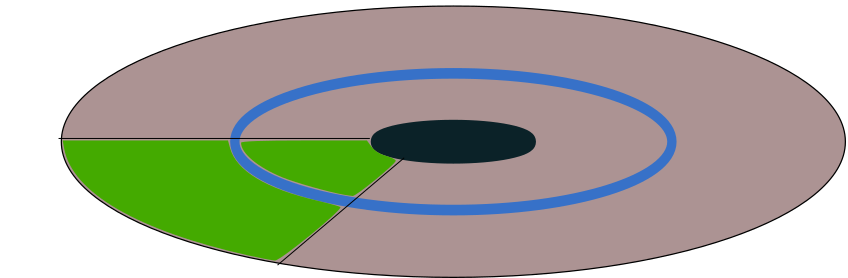
\includegraphics[width=0.8\linewidth]{fig3/secteur}
    \center{Un secteur}
  \end{figure}
\end{frame}

\begin{frame}
  \frametitle{\insertsubsection}
  Le secteur d'une piste \ding{212} un \alert{bloc de données}
  \begin{figure}
    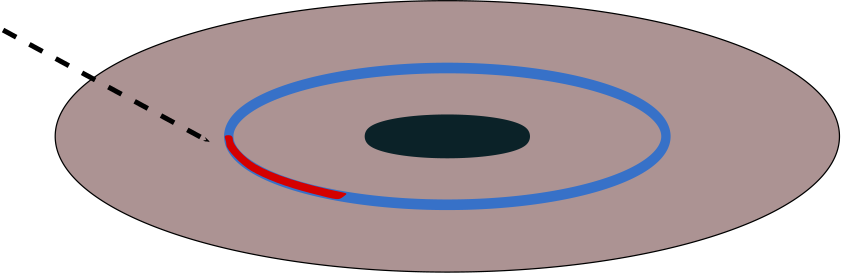
\includegraphics[width=0.8\linewidth]{fig3/bloc}
    \center{Un bloc}
  \end{figure}
\end{frame}

\begin{frame}
  \frametitle{\insertsubsection}
  Le déplacement de la tête et la rotation du disque permettent d'accéder aux
  différents blocs~:
  \vspace{0.5cm}
  \begin{itemize}
  \item[\ding{212}] changement de piste par \alert{mouvement} de la tête   
  \item[\ding{212}] changement de secteur par \alert{rotation} du disque
  \end{itemize}
  \vspace{0.5cm}

  Les disques tournent très rapidement autour d'un axe
  \begin{itemize}
  \item milliers de tours par minute
  \end{itemize}
\end{frame}

\subsection{Avec plusieurs plateaux}
\begin{frame}
  \frametitle{\insertsubsection}
  \begin{figure}
    \includegraphics[width=0.8\linewidth]{fig3/harddisk.png}
  \center{Un axe, un bras, plusieurs plateaux}
  \end{figure}
\end{frame}

\begin{frame}
\frametitle{\insertsubsection}
\large{Un axe, un bras, plusieurs plateaux
  \begin{itemize}
  \item plusieurs têtes de lecture 
  \item[\ding{212}] liées entre elles (un seul bras)
  \item[\ding{212}] une seule tête peut lire ou écrire à un moment donné. 
  \item rotation de tous les plateaux
\end{itemize}}
\end{frame}

\begin{frame}
  \frametitle{\insertsubsection}
  \begin{figure}
    \includegraphics[width=0.8\linewidth]{fig3/dd1.png}
  \end{figure}
 Ensemble des données stockées verticalement sur une même piste de chaque plateau~:
 un \alert{cylindre}
\end{frame}

\begin{frame}
\frametitle{\insertsubsection}
Changer de cylindre \ding{212} \alert{déplacer} le bras 
\begin{itemize}
\item déplace toutes les têtes de lecture
\item mouvement mécanique
\end{itemize}

Changer de tête de lecture
\begin{itemize}
\item sélectionner une tête
\item commutation électronique
\end{itemize}
\end{frame}

\subsection{Temps d'accès}
\begin{frame}
  \frametitle{\insertsubsection}
  Accéder à un bloc 
  \begin{itemize}
  \item[\ding{212}] déplacement de la tête
  \item[\ding{212}] rotation du disque
  \end{itemize}
  \vspace{0.5cm}
  
  Délais = rotation + déplacement du bras
  \begin{itemize}
  \item plus le bloc est ``loin'' plus le délais est long
  \item le plus lent~: déplacement de la tête
  \end{itemize}
  \vspace{0.5cm}
  \underline{A retenir}~: temps d'accès \alert{non uniforme}
\end{frame}

\begin{frame}
  \frametitle{\insertsubsection}
  \large
  \alert{Idée~:} minimiser les déplacements de la tête
  \vspace{0.5cm}
  \begin{itemize}
  \item principe de \alert{localité}
  \item[\ding{212}] grouper les données par \alert{cylindre}
  \end{itemize}
  \normalsize
\end{frame}

\subsection{Quelques chiffres}
\begin{frame}
  \frametitle{Quelques chiffres}
  \large
  \begin{tabular}{ll}
    couche magnétique & 10-20 nm \vspace{0.2cm}\\
    vitesse de rotation & 5400-15000 tours/min \vspace{0.2cm}\\
    capacité & 120 GB -2 TB \vspace{0.2cm}\\
    temps d'accès & 2-15 ms \vspace{0.2cm}\\
    vitesse de transfert & 70 Mo/sec (7200 t/min) 
  \end{tabular}
  \normalsize
\end{frame}

\subsection{Bilan}
\begin{frame}
\frametitle{\insertsubsection}
\underline{Technologie}
\begin{itemize}
\item enregistrement magnétique
\item cylindres, pistes, secteurs, blocs
\item déplacement de pièces mécaniques
\end{itemize}
\vspace{0.5cm}
\underline{Conséquences}
\begin{itemize}
\item \alert{lenteur relative}
\item \alert{temps d'accès aux blocs non uniforme}
\item[\ding{212}] répercussion sur le temps des E/S sur disque
\end{itemize}
\end{frame}


%%%%%%%%%%%%%%%%%%%%%%%%%%%%%%
\section{Gestion des entrées/sorties sur disque}

\begin{frame}    
  \frametitle{\insertsection}
  \underline{Idée}: minimiser les déplacements entres les lectures/écritures\\
  \vspace{0.5cm}
  \underline{Système monotâche}
  \begin{itemize}
  \item on déplace la tête à la demande là où on en a besoin
  \item performances meilleures si les blocs d'un même fichier sont regroupés
  \item[\ding{212}] \alert{défragmentation} du système de fichiers    
  \end{itemize}
\end{frame}

\begin{frame}
  \frametitle{E/S sur système multitâche}
  Sur système multitâche, plusieurs processus demandent des E/S
  \begin{itemize}
  \item plusieurs demandes en attente
  \item implique des déplacements de tête plus ou moins importants 
  \item dépend de la position actuelle de la tête et de la position voulue  
  \end{itemize}
  \vspace{0.5cm}
  Quelle demande servir en premier~?\\
\underline{Pb}~: \alert{ordonnancement} des mouvements du bras
\end{frame}

\subsection{E/S~: premier arrivé, premier servi}
\begin{frame}
  \frametitle{\insertsubsection}
  Politique premier arrivé, premier servi\\
  \vspace{0.5cm}
  \underline{Exemple}: 3 processus
  \begin{itemize}
  \item P1 : lit les blocs 100, 101, 102 ...
  \item P2 : lit les blocs 200, 201, 202 ...
  \item P3 : lit les blocs 500, 501, 502 ...
  \end{itemize}
  \vspace{0.5cm}
  \pause
  \underline{Déroulement}:
  \pause 100, 
  \pause 200, 
  \pause 500, 
  \pause 101, 
  \pause 201, 
  501, 102, 202, 502 ...
\end{frame}

\begin{frame}
  \frametitle{\insertsubsection}
  \large
  Politique premier arrivé, premier servi 
  \begin{itemize}
  \item \alert{simple} à mettre en \oe{}uvre
  \item \alert{équitable}
  \item mais \alert{pas efficace}
  \end{itemize}
  \normalsize
\end{frame}


\subsection{E/S : plus court déplacement}
\begin{frame}
\frametitle{\insertsubsection}
\alert{Plus court déplacement}, on sert d'abord le plus prêt.\\
\vspace{0.5cm}
\underline{Exemples}: 3 processus
\begin{itemize}
\item P1 : lit les blocs 100, 101, 102 ...
\item P2 : lit les blocs 200, 201, 202 ...
\item P3 : lit les blocs 500, 501, 502 ...
\end{itemize}
\pause
\vspace{0.5cm}
\underline{Déroulement}:
\pause 100, 
\pause 200, 
\pause 101, 
\pause 201, 
\pause 102, 202, ...
\end{frame}

\begin{frame}
  \frametitle{\insertsubsection}
  \large
  Politique du déplacement le plus court
  \begin{itemize}
  \item \alert{simple} à mettre en \oe{}uvre
  \item \alert{efficace} 
  \item \alert{pas équitable}
  \end{itemize}
  \normalsize
\end{frame}

\subsection{E/S : politique de l’ascenseur}
\begin{frame}
  \frametitle{Quel compromis possible?}
  Compromis entre équité et efficacité\\
  \ding{212} politique de l'\alert{ascenseur}\\
  \vspace{0.5cm}
  \underline{Idée}: on traite de proche en proche dans une même direction, 
  arrivé ``au bout'', on fait la même chose dans l'autre sens.
\end{frame}

\begin{frame}
  \frametitle{\insertsubsection}
  \underline{Exemples~:} 3 processus
  \begin{itemize}
  \item P1 : lit les blocs 100, 101, 102 ...
  \item P2 : lit les blocs 200, 201, 202 ...
  \item P3 : lit les blocs 500, 501, 502 ...
  \end{itemize}
  \vspace{0.5cm} \pause
  \underline{Déroulement}:
  \begin{itemize}
  \item \pause ($\Uparrow$) \pause  100, \pause 200, \pause 500, 
  \item \pause ($\Downarrow$) \pause 201, \pause 101, 
  \item \pause ($\Uparrow$) 202, 501,
  \item \pause  ($\Downarrow$) 203, 102,
  \item \pause ($\Uparrow$) 204, 502  
  \item ($\Downarrow$) ...
  \end{itemize}
\end{frame}

\begin{frame}
  \frametitle{\insertsubsection}
  \large
  Politique de l'ascenseur
  \begin{itemize}
  \item \alert{assez équitable}
  \item \alert{assez efficace}
  \end{itemize}
  
  \vspace{0.5cm}
  \underline{Problème}: que faire pour les \alert{requêtes urgentes}~?
  \normalsize
\end{frame}

\subsection{E/S : Deadline driven disk scheduler}
\begin{frame}
\frametitle{\insertsubsection}
Politique \alert{deadline driven scheduling}\\
\vspace{0.2cm}
\underline{Idée}: on dispose d'un \alert{délai maximum} pour servir une requête\\
\vspace{0.5cm}
Requête urgente $\Leftrightarrow$ délai dépassé
\vspace{0.5cm}

Si il y a des requêtes \alert{urgentes} 
\begin{itemize}
\item traitées en priorité
\item \alert{dans l'ordre d'apparition}
\end{itemize}
Sinon, requêtes normales
\begin{itemize}
\item  \alert{plus court déplacement}
\end{itemize}
\end{frame}

\begin{frame}
\frametitle{\insertsubsection}
Politique deadline driven scheduling
\begin{itemize}
 \item \alert{efficace}
 \item et \alert{équitable}
\pause \item ... et breveté
\end{itemize}
\vspace{0.5cm}
\alert{United States Patent 5787482} (1998)\\
\vspace{0.5cm}
\texttt{\small\underline{Subject}: Deadline driven disk scheduler method and
  apparatus with thresholded most urgent request queue scan window}
\end{frame}


\subsection{Bilan~: ordonnancement d'E/S}
\begin{frame}
  \frametitle{\insertsubsection}
  \underline{Problème}~: \alert{temps d'accès non uniforme}\\
  \structure{Compromis} à trouver entre 
  \begin{itemize}
  \item \alert{efficacité}
  \item \alert{équité}
  \end{itemize}
  Quelques heuristiques pour l'ordonnancement
  \begin{itemize}
  \item premier arrivé, premier servi
  \item plus court déplacement
  \item ascenseur
  \item \alert{deadline scheduling}
  \item ...
  \end{itemize}
\end{frame}

%%%%%%%%%%%%%%%%%%%%%%%%%%%%%%%%%%%%%%%%%
\section{Les systèmes RAID}
\subsection{Objectifs des systèmes RAID}
\begin{frame}
  \frametitle{\insertsubsection}
  \underline{Constat initial}: marché du disque dur partagé entre les secteurs
  \begin{itemize}
  \item \alert{professionnel} 
    \begin{itemize}
    \item disques de grande capacité
    \item fiables, 
    \item performants, 
    \item[\ding{212}] \alert{chers}
    \end{itemize}
  \item \alert{ particuliers}
    \begin{itemize}
    \item petits disques
    \item bon marché
    \end{itemize}
  \end{itemize}
\end{frame}

\begin{frame}
  \frametitle{\insertsubsection}
  \underline{Idée}: \alert{grouper des disques} bon marché pour 
  \begin{itemize}
  \item étendre la \alert{capacité}
  \item améliorer la \alert{fiabilité}
  \item gagner en \alert{performances}
  \item à moindre coût
  \end{itemize}
\end{frame}

\begin{frame}
  \frametitle{Système RAID}
  \large
  \begin{tabular}{r|c|l}
    $\Rightarrow$ & R&edundant \\ & A&rray \\ of &I&nexpensive \\ & D&isks
    \end{tabular}
  \normalsize
  \newline\\
  \vspace{0.5cm}
  Baisse des prix\\ \ding{212} \emph{Redundant Array of \alert{Independent} Disks}\\
  \vspace{0.5cm}
  Implémentation matériel ou logiciel\\
  \vspace{0.5cm}
  Différents systèmes RAID
\end{frame}

\subsection{Les systèmes RAID usuels}
\begin{frame}
  \frametitle{NRAID (ou JBOD)~: concaténation}
  Répartition, pas de redondance
  \begin{itemize}
  \item NRAID is \alert{Not R}AID, 
  \item JBOD~: \alert{Just a Bunch of Disks}
  \end{itemize}
  \begin{figure}
    \includegraphics[width=0.8\linewidth]{fig3/NRAID}
  \end{figure}
\end{frame}

\subsection[RAID 0]{RAID 0~: agrégation par bandes (stripping)}
\begin{frame}
  \frametitle{\insertsubsection}
  \alert{Répartition} de la charge, \alert{lectures simultanées} sur plusieurs disques
  \begin{itemize}
  \item \underline{exp}: lecture/écriture de 2, 6 et 10
  \end{itemize}
  \begin{figure}
    \includegraphics[width=0.8\linewidth]{fig3/RAID0}
  \end{figure}
\end{frame}

\begin{frame}
  \frametitle{\insertsubsection}
  Anticipation des lectures suivantes
  \begin{itemize}
  \item demande de lecture 7, possibilité de \alert{lecture
    anticipée} de 8 et 9 dans le même temps
  \end{itemize}
  \begin{figure}
    \includegraphics[width=0.8\linewidth]{fig3/RAID0}
  \end{figure}
\end{frame}



\subsection{RAID 1~: miroir}
\begin{frame}
  \frametitle{\insertsubsection}
  \alert{Redondance} des données, fiabilité
  \small
  \begin{itemize}
  \item défaillance d'un disque \ding{212} données sur le miroir
  \item \alert{répartition} des lectures
  \item \alert{l'écriture} doit se faire en parallèle
  \end{itemize}
  \normalsize
  \begin{figure}
    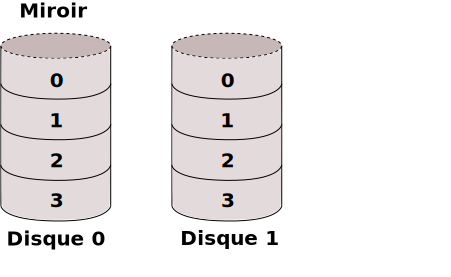
\includegraphics[width=0.75\linewidth]{fig3/RAID1}
  \end{figure}
\end{frame}


\subsection{RAID 4 : agrégation par bandes avec parité}
\begin{frame}
  \frametitle{\large{\insertsubsection}}
  \underline{Objectif}~: \alert{reconstitution} d'un disque défectueux
  \begin{itemize}
  \item généralisation de l'idée de \alert{miroir}
  \item utilise les propriétés du \alert{ou-exclusif}
  \end{itemize}
  \begin{figure}
    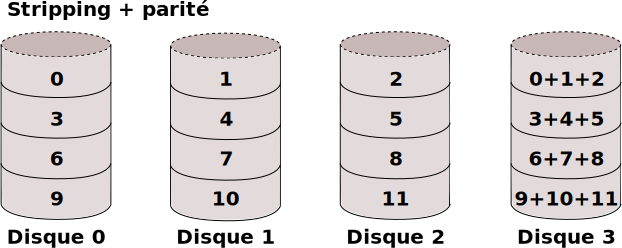
\includegraphics[width=1\linewidth]{fig3/RAID4}
  \end{figure}
\end{frame}


\begin{frame}
\frametitle{\large{\insertsubsection}}
  \begin{figure}
    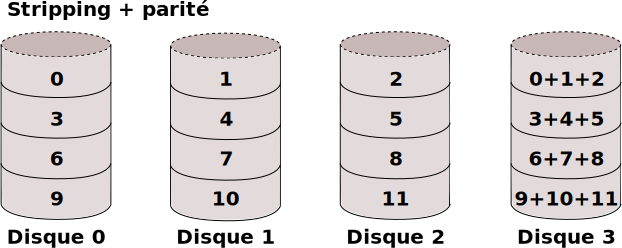
\includegraphics[width=1\linewidth]{fig3/RAID4}
  \end{figure}
  \center{
    $a \oplus b \oplus c \oplus \ldots = 0  $ \\
    $ \Leftrightarrow $ \\
    $a = b \oplus c \oplus \ldots $\\
  }
\end{frame}



\begin{frame}
\frametitle{\large{\insertsubsection}}
  \begin{figure}
    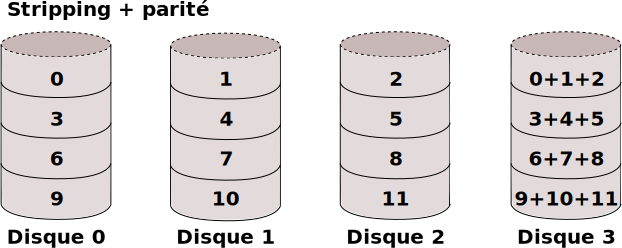
\includegraphics[width=1\linewidth]{fig3/RAID4}
  \end{figure}
  Lecture en parallèle\\
  \alert{Goulet d'étranglement en écriture}
  \begin{itemize}
  \item accès au disque de parité
  \end{itemize}
\end{frame}

\subsection[RAID 5]{RAID 5~: agrégation par bandes avec parité répartie}
\begin{frame}
\frametitle{\insertsubsection}
\underline{Objectif}: fiabilité, performances
\begin{itemize}
\item répartition de la charge en écriture
\end{itemize}
\begin{figure}
  \includegraphics[width=1\linewidth]{fig3/RAID5}
\end{figure}
\end{frame}

\subsection{Combinaisons de RAID}
\begin{frame}
  \frametitle{Combinaisons de RAID}
  \underline{Idée}: combiner les systèmes
  \begin{itemize}
  \item combinaison des avantages
  \item au prix de disques supplémentaires
  \end{itemize}
  \vspace{0.5cm}

  Exemples~: 
  \begin{itemize}
  \item \alert{RAID 1+0}~: stripping sur disques en miroir
  \item \alert{RAID 10}~: miroir de grappes RAID 1
  \item \alert{RAID 51}~: miroir de grappes RAID 5
  \end{itemize}
\end{frame}


\begin{frame}
\frametitle{RAID 0+1}
\begin{figure}
  \includegraphics[width=\linewidth]{fig3/RAID0+1}
  \center{miroir de grappes RAID 0}
\end{figure}
\end{frame}

\begin{frame}
\frametitle{RAID 10}
\begin{figure}
  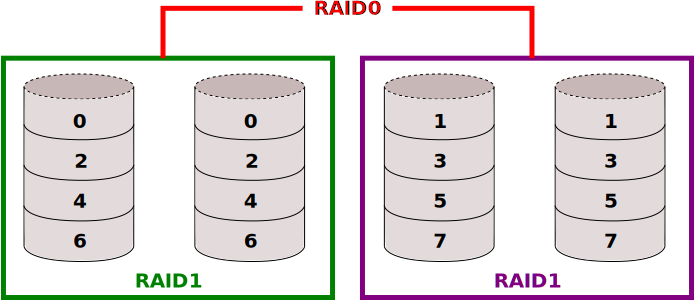
\includegraphics[width=\linewidth]{fig3/RAID10}
  \center{RAID 0 sur des disques en miroir}
\end{figure}
\end{frame}

\begin{frame}
\frametitle{RAID 51}
\vspace{-0.2cm}
\begin{figure}
  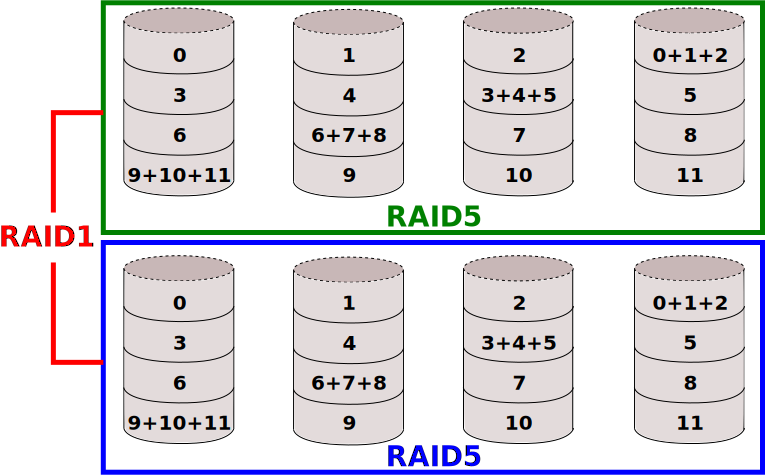
\includegraphics[width=\linewidth]{fig3/RAID51}
  \center{\alert{Miroir} de \alert{grappes RAID 5}}
\end{figure}
\end{frame}

\subsection{Conclusion}
\begin{frame}
  \frametitle{\insertsubsection}
  \large
  Objectifs des systèmes RAID~: 
  \begin{itemize}
  \item capacité, fiabilité, performances
  \end{itemize}
  \vspace{0.5cm}
  Diverses techniques~: 
  \begin{itemize}
  \item duplication, \emph{striping}, parité, répartition, ...
  \end{itemize}
  \vspace{0.5cm}
  \ding{212} Objectifs atteints par combinaison
\end{frame}


%% \begin{frame}
%% \frametitle{\insertsubsection}
%% Choix d'une configuration RAID fonction d'objectifs définis\\
%% Serveurs de fichier RAID technologie indispensable\\
%% ... ne dispense pas des sauvegardes
%% \end{frame}

\end{document}

% LocalWords:  blue ASR width fichiers-images beamer currentsection Michel PCTE
% LocalWords:  hideothersubsections Billaud Let's Operating System Fisrt-fit nm
% LocalWords:  Best-fit Swapping swapping MMU Memory Managment t-il sys GB TB
% LocalWords:  électro-aimant Pb uvre Deadline driven disk scheduler deadline
% LocalWords:  scheduling United States Subject method and apparatus with most
% LocalWords:  thresholded request scan window d'E edundant rray of nexpensive
% LocalWords:  isks Redundant Array Independent Disks NRAID JBOD is Not AID exp
% LocalWords:  Just Bunch ou-exclusif striping
